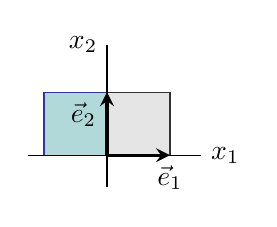
\begin{tikzpicture}[scale=0.8]

    \coordinate (O) at (0,0);  % variable for origin
       
    % grey box
        \filldraw[
        draw=black!80,fill=black!10]          
            (0,1) 
            -- (1,1)
            -- (1,0)
            -- (O)
            -- cycle;
            
    % blue box
        \filldraw[
        draw=DarkBlue!80,fill=Teal!30]          
            (-1,0) 
            -- (-1,1)
            -- (0,1)
            -- (O)
            -- cycle;            
    % axes
    \draw[-, thin,black] (-1.25,0) -- (1.5,0) node[anchor=west] {$x_1$};
    \draw[-, thin,black] (0,-0.5) -- (0.0,1.75) node[anchor=east] {$x_2$};
    
    % coordinate vectors            
    \draw[->,Black,very thick,-stealth,rotate=0] (O) -- (0,1) node[anchor=north east] {$\vec e_2$}; 
    \draw[->,Black,very thick,-stealth,rotate=0] (O) -- (1,0) node[anchor=north] {$\vec e_1$}; 
    
\end{tikzpicture}